\documentclass[11pt,a4paper]{article}
\usepackage[utf8]{inputenc}
\usepackage[T1]{fontenc}
\usepackage{amsfonts}
\usepackage[french]{babel}
\frenchbsetup{StandardLists=true} % à inclure si on utilise \usepackage[francais]{babel}
\usepackage{enumitem}
\usepackage{amssymb}
\usepackage{amsmath}
\usepackage{parskip}
\usepackage[left=2cm,right=2cm,top=2cm,bottom=2cm]{geometry}
\usepackage{multirow}
\usepackage[dvipsnames]{xcolor}

\usepackage[T1]{fontenc}
\usepackage{fouriernc}
\usepackage{graphicx}

\usepackage{setspace}
\singlespacing

\usepackage{pstricks}
\usepackage{xkeyval}
\usepackage{pst-labo}


\usepackage{multicol}
\usepackage{caption}
\usepackage{fancyhdr}
\pagestyle{fancy}
\renewcommand\headrulewidth{1pt}
\fancyhead[L]{Lycée Denis Diderot }
\fancyhead[R]{Classe de Terminale}
\setcounter{page}{7}\fancyfoot[C]{page \thepage}
\fancyfoot[R]{Année 2025 2026}
\fancyfoot[L]{Alexis RUIZ}
\usepackage{multirow,tabularx,booktabs}
\newcommand{\cadreblanc}[1]{%
\medskip\framebox[\linewidth][c]{%
\rule{0mm}{#1mm}}\par
\medskip}

\usepackage{awesomebox}
\setlength{\aweboxvskip}{0mm}
\usepackage{pifont}
\usepackage{chemmacros}
\usepackage{chemist}
\chemsetup{modules=all}

\renewcommand{\arraystretch}{2}
\newcommand*\acocher{\quitvmode{\fboxsep0pt \fboxrule0.8pt \fbox{\vrule height1.8ex depth.1ex width0pt \vrule height0pt depth0pt width1.9ex }}}
\usepackage{colortbl}

\newcommand{\defproblem}{\awesomebox[black]{2pt}{\rotatebox{90}{\large{\textbf{Problématique}}}}{black}}
\newcommand{\defconclusion}{\awesomebox[black]{2pt}{\rotatebox{90}{\Large{\textbf{Conclusion}}}}{black}}
\newcommand{\defbox}{\awesomebox[black]{2pt}{
\includegraphics[scale=0.5]{images/appel exam.png}}{black}}


\frenchbsetup{StandardLists=true}
\begin{document}



\begin{center}
\LARGE{Evaluation- Prévoir une réaction d'oxydo-réduction}\\[5mm]
\end{center}
\normalsize
\hrule 
NOM : \\[5mm]
Prénom :\\

\hrule
\vspace {8 mm}


\textbf{Exercice 1 : Cases à cocher}

\ding {202} Indiquer pour chacune des affirmations si elle est vrai ou elle est fausse en cochant la case correspondante. \\[0.3cm]

 
\renewcommand{\arraystretch}{1.5}
\begin{center}
\begin{tabularx}{15cm}{|p{11cm}|X|X|}
    \hline
    Affirmation & Vraie & Fausse\\
    \hline
     Une réaction d'oxydo-réduction est un échange de protons & &\\
    \hline
     Une oxydation est une perte d'électrons & &\\
    \hline
    Une réduction est un gain d'électrons & &\\
    \hline
    Un oxydant perds des électrons & &\\
    \hline
    Le métal cuivre est un réducteur &  &\\
    \hline
\end{tabularx}
\end{center}

\vfill
\ding {203} Les ions \ch{Cu \pch[2]} réagissent avec le métal zinc \ch{Zn} pour donner un dépôt  de cuivre métallique \\ et des ions \ch{Zn \pch[2]}\\[0.5 cm]
\textbf{Cocher la case correspondante à toute équation exacte :} \\[0.5cm]
\begin{center}
\begin{tabularx}{12cm}{p{8cm}X X}
 
   
      L' ion \ch{Cu \pch[2]} est l'oxydant le plus fort  & \acocher ~~Oui & \acocher ~~Non\\
 
     L' ion \ch{Zn \pch[2]} est l'oxydant le plus fort & \acocher ~~Oui & \acocher ~~Non\\
 
  
    le métal cuivre est le réducteur le plus fort & \acocher ~~Oui & \acocher ~~Non\\
  

    Le métal zinc est le réducteur le plus fort  & \acocher ~~Oui & \acocher ~~Non\\

\end{tabularx}
\end{center}

\vfill 

\ding {204}  Les ions \ch{Cu \pch[2]} réagissent avec le métal fer \ch{Fe} pour donner un dépôt\\ de cuivre métallique et des ions \ch{Fe \pch[2]}\\[0.5 cm]
\textbf{Cocher la case correspondante à toute équation exacte : } \\[0.5cm]

 \begin {multicols}{2}
 	\acocher ~~\ch{Cu \pch[2] + 2 e \mch[] -> Cu} \\[2mm]
 	\acocher ~~\ch{Fe \pch[2] + 2 e \mch[] -> Fe} \\[2mm]
 	\acocher ~~\ch{Cu \pch[2] + Fe -> Cu + Fe \pch[2]} \\[2mm]
 	\acocher ~~\ch{Cu -> Cu \pch[2] + 2 e \mch[] } \\[2mm]
  	\acocher ~~\ch{Fe -> Fe\pch[2] + 2 e \mch[] } \\[2mm]
  	\acocher ~~\ch{Cu  + Fe \pch[2]-> Cu \pch[2] + Fe } \\[2mm]

 \end {multicols}


\vfill 


\newpage


\textbf{Exercice 2 : QCM}~~Parmi les trois propositions, entourer la bonne réponse. 
\begin{center}
\renewcommand{\arraystretch}{2.5}
\begin{tabular}{|>{\columncolor{Peach}}m{4mm}|p{4.5cm}||m{3.5cm}|m{3.5cm}|m{3.5cm}|}
    \hline
    \ding{202} & Au cours d'une réaction d'oxydo-réduction, l'oxydant   & perd des protons & perd des électrons & gagne des électrons \\
    \hline
    
    \ding{203} & Dans quel cas l'ion en solution ne se dépose-t-il pas sur la lame métallique  & ~~~~~~~~\raisebox{-.7\height}{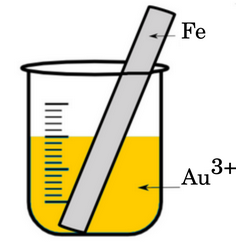
\includegraphics[scale=1]{images/QCm21.png}}& ~~~~~~~~\raisebox{-.7\height}{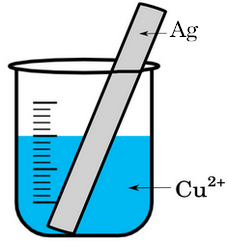
\includegraphics[scale=1.05]{images/QCm22.png}} & ~~~~~~~~\raisebox{-.7\height}{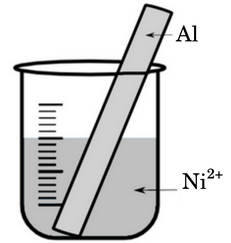
\includegraphics[scale=1]{images/QCm23.png}} \\
    \hline
    \ding{204} & Une réduction est   & une perte d'électrons & un gain d'électrons & une perte de neutrons \\
    \hline
    \ding{205} & Au cours d'une réaction chimique l' ion Argent (\ch{Ag\pch[]})  se transforme en atome d'argent (\ch{Ag}) , on dit  & qu'il s'oxyde  & qu'il se protège & qu'il se réduit \\
    \hline
    \ding{206} & Lors de la réduction des ions Cuivre ceux ci  &  gagnent deux \ch{e\mch[]} & gagnent un \ch{e\mch[]}& perdent trois \ch{e\mch[]}\\
    \hline
    \ding{207} & les ions chrome (\ch{Cr\pch[3]}) sont plus oxydant que les ions aluminium (\ch{Al\pch[3]})  qu'elle est l'équation possible& $$\ch{Cr}+ \ch{Al\pch[3]}\longrightarrow \ch{Al} + \ch{Cr\pch[3]}$$  &  $$\ch{Al\pch[3]}+ \ch{Cr\pch[3]}\longrightarrow \ch{Al}+ \ch{Cr}$$ & $$\ch{Al} + \ch{Cr\pch[3]}\longrightarrow \ch{Cr}+ \ch{Al\pch[3]}$$\\
    \hline
    \ding{208} & Que faut-il faire pour écrire l'équation bilan de ~~~~~~~~ $ \ch{Al}\longrightarrow \ch{Al\pch[3]}+ 3\ch{e\mch[]}$ et $ \ch{Zn \pch[2]}+2\ch{e\mch[]}\longrightarrow \ch{Zn}$  & additionner membres à membres  &  multiplier par 3 la première demi-équation, multiplier par 2 la seconde demi-équation puis additionner membre à membre & multiplier par 2 la première demi-équation, multiplier par 3 la seconde demi-équation puis additionner membre à membre \\
    \hline
   
\end{tabular}
\end{center}



\newpage

\textbf{Exercice 3 :} Dans un bêcher on plonge un métal dans une solution ionique métallique. 
 Pour chacune des expérience, indiquer s'il y a une réaction, dans ce cas écrire les demi-équations d'oxydo-réduction, puis l'équation de réaction.Si la réaction n'a pas lieu, pas besoin d'écrire les équations.   \\[5mm]

\textbf{Exp~~\ding{202} :} On introduit de la grenaille d'argent (\ch{Ag}) dans une solution contenant des ions cuivre (\ch{Cu\pch[2]})

\begin{figure}[h]
\begin{minipage}{0.2\textwidth}
\begin{center}
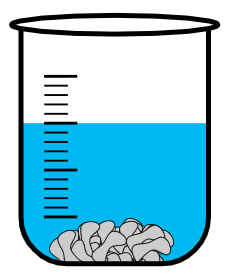
\includegraphics[scale=0.25]{images/sol cu metal zn.png} 
\end{center}
\end{minipage}%
\begin{minipage}{0.8\textwidth}
La réaction a-t-elle lieu ? $\Box$ oui $\Box$ non \\[2mm]
Écrire les deux demi équations correspondantes à cette réaction. \\[2mm]
\LARGE{\fbox{$~~~~~~~~ ~~~~~~\longrightarrow~~~~~~~~~~ ~~~~~~~~$} ~~~~~~~~ \fbox{$~~~~~~~~ ~~~~~~~~ \longrightarrow ~~~~~~~~~~~~ $}}\\[2mm]
\normalsize
Écrire l'équation de la réaction. \\[2mm]
\fbox{\LARGE {$~~~~~~~~~~+ ~~~~~~~~~~ \longrightarrow~~~~~~~~~~+ ~~~~~~~~ $}}\\

\end{minipage}
\end{figure}

\vspace {5mm}

\textbf{Exp~~\ding{203} :} On introduit de la grenaille de Zinc (\ch{Zn)} dans une solution contenant des ions platine (\ch{Pt\pch[2]})
\begin{figure}[h]
\begin{minipage}{0.7\textwidth}
La réaction a-t-elle lieu ? $\Box$ oui $\Box$ non \\[2mm]
Écrire les deux demi équations correspondantes à cette réaction. \\[2mm]
\LARGE{\fbox{$~~~~~~~~ ~~~~~~\longrightarrow~~~~~~~~~~ ~~~~~~~~$} ~~~~~~~~ \fbox{$~~~~~~~~ ~~~~~~~~ \longrightarrow ~~~~~~~~~~~~ $}}\\[2mm]
\normalsize
Écrire l'équation de la réaction. \\[2mm]
\fbox{\LARGE {$~~~~~~~~~~+ ~~~~~~~~~~ \longrightarrow~~~~~~~~~~+ ~~~~~~~~ $}}\\

\end{minipage}
\begin{minipage}{0.3\textwidth}
\begin{center}
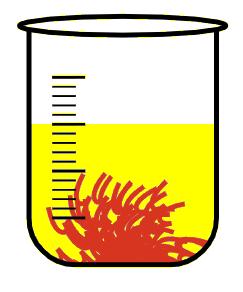
\includegraphics[scale=0.25]{images/sol pb metal cu.png} 
\end{center}
\end{minipage}%
\end{figure}

\vspace {5mm}

\textbf{Exp~~\ding{204} :} On introduit de la grenaille d'aluminium (\ch{Al}) dans une solution contenant des ions étain (\ch{Sn\pch[2]})
\begin{figure}[h]
\begin{minipage}{0.3\textwidth}
\begin{center}
\includegraphics[scale=0.25]{images/sol etain metal Al.png} 
\end{center}
\end{minipage}%
\begin{minipage}{0.8\textwidth}
La réaction a-t-elle lieu ? $\Box$ oui $\Box$ non \\[2mm]
Écrire les deux demi équations correspondantes à cette réaction. \\[2mm]
\LARGE{\fbox{$~~~~~~~~ ~~~~~~\longrightarrow~~~~~~~~~~ ~~~~~~~~$} ~~~~~~~~ \fbox{$~~~~~~~~ ~~~~~~~~ \longrightarrow ~~~~~~~~~~~~ $}}\\[2mm]
\normalsize
Écrire l'équation de la réaction. \\[2mm]
\fbox{\LARGE {$~~~~~~~~~~+ ~~~~~~~~~~ \longrightarrow~~~~~~~~~~+ ~~~~~~~~ $}}\\

\end{minipage}
\end{figure}

\vspace {5mm}

\textbf{Exp~~\ding{205} :} On introduit de la grenaille de magnésium (\ch{Mg})  dans une solution contenant des ions fer (\ch{Fe\pch[2]})
\begin{figure}[h!]
\begin{minipage}{0.7\textwidth}
La réaction a-t-elle lieu ? $\Box$ oui $\Box$ non \\[2mm]
Écrire les deux demi équations correspondantes à cette réaction. \\[2mm]
\LARGE{\fbox{$~~~~~~~~ ~~~~~~\longrightarrow~~~~~~~~~~ ~~~~~~~~$} ~~~~~~~~ \fbox{$~~~~~~~~ ~~~~~~~~ \longrightarrow ~~~~~~~~~~~~ $}}\\[2mm]
\normalsize
Écrire l'équation de la réaction. \\[2mm]
\fbox{\LARGE {$~~~~~~~~~~+ ~~~~~~~~~~ \longrightarrow~~~~~~~~~~+ ~~~~~~~~ $}}\\

\end{minipage}
\begin{minipage}{0.3\textwidth}
\begin{center}
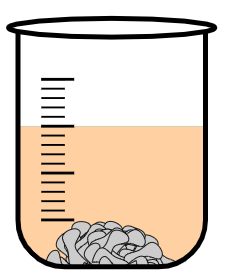
\includegraphics[scale=0.25]{images/sol fer metal zinc.png} 
\end{center}
\end{minipage}%
\end{figure}







\end{document}